\begin{savequote}[8cm]
La fisica è diventata così potente e ricca da poter nuovamente introdurre nei propri modelli la complessità e il disordine, ciò che Galileo era stato costretto a escludere.

Physics has become so powerful and rich to be able to re-introduce complexity and disorder in its models, which is what Galileo was forced to leave behind.
\qauthor{--- Giorgio Parisi}
\end{savequote}


\chapter{\label{ch:4-KF-NDGArLite}Kalman Filter reconstruction for ND-GAr-Lite}
\minitoc

\section{Introduction}
ND-GAr-Lite was a proposed temporary muon spectrometer  for the DUNE ND complex, to be used during Phase-I of the experiment. As described in Section \ref{Sec: DUNE-GArLite} the key design principle behind the detector was to include the structural components of ND-GAr, but to exclude the active detector elements: the gas TPC and the ECAL. In their place a simple tracker composed of segmented tracking planes would be built. Significant effort was dedicated to this design by the ND-GAr group, which was able to produce official geometries for the detector and code which allowed to fully simulate the passage of particles through it, down to the signal formation, and track finding and reconstruction.

While a full simulation for ND-GAr-Lite was available at the time of the writing of this thesis, it was known that many aspects were not mature. In particular the track reconstruction algorithm was known not to be at a state-of-the-art level. No treatment of energy loss or multiple scattering was put in place and no estimate of the uncertainties from the measurement was produced by the algorithm.

As a key part of this thesis project, a collaboration with experts from the ALICE experiment tracking group was established to produce a Kalman Filter based on the one used for the ALICE TPC (see Chapter \ref{ch:5-KF-NDGArToy} for a full description). This new algorithm was set to improve on the existing one and fit the needs of both the new geometry of the ALICE detector as well as ND-GAr. In this context, an additional goal of this thesis project became to produce a similar algorithm, also based on the pre-existing ALICE Kalman Filter, that could be applied to ND-GAr-Lite's tracker. 

The first step in the development of the algorithm, consisted in creating a simple Toy Monte Carlo simulation which allowed for a high degree of control over many aspects of particle propagation and signal formation. This was achieved by developing many aspects of the simulation modularly and somewhat independently from one another. Most of the development stage in the algorithm's life consisted in producing different samples with this Toy Monte Carlo tool and then testing the performance of the algorithm and whether it conformed to expectations. Once the Kalman Filter was thought to be at a good level of maturity, it was tested on the more complete simulation already available from the ND-GAr group.

This Chapter will be divided as follows: in Sec. \ref{Sec:KFLite} we introduce the Kalman Filter algorithm developed for ND-GAr-Lite; in Sec. \ref{Sec:GArSoft_Lite} we give a full description of the simulation software developed by the ND-GAr group; in Sec. \ref{Sec:ToySim-Lite} we describe the Toy Monte Carlo tool specifically developed for the testing of the Kalman Filter; in Sec. \ref{Sec:ToyMCTests-Lite} we present some selected results from the tests done using the Toy Monte Carlo tool; in Sec. \ref{Sec:MC-Studies-Lite} we show the performance of the algorithm when applied to the more complete simulation developed by the ND-GAr group and we compare with the results obtained with the previously existing algorithm.

\section{The Kalman Filter Applied to ND-GAr-Lite}
\label{Sec:KFLite}
The Kalman Filter developed for ND-GAr-Lite was largely based on the parametrization utilized by the ALICE collaboration for their own TPC Kalman Filter, which can be considered the state of the art in the field ~\cite{Ivanov:2003yr, Arslandok:2022dyb}. The code produced to apply and test the custom Kalman Filter, however was largely produced as a custom tool to accommodate the peculiarities of ND-GAr-Lite's tracking system which has little in common with a gas TPC such as ALICE. The Kalman Filter algorithm developed for GArLite will be referred to as \texttt{KF-Lite}. For a brief overview of the Kalman Filter technique applied to track reconstruction see Section where we also define the nomenclature used to describe \texttt{KF-Lite}.

We assume that an ideal magnetic field is applied along the direction perpendicular to the neutrino beam which is identified by the coordinate $z$. The $x$ coordinate identifies the horizontal direction, while the $y$ coordinate identifies the vertical.  The spatial information in the $zy$ plane is assumed to be given by the detector's tracking planes as will be discussed in more detail in Section[ref-needed]. The information regarding the $x$ coordinate is given by the central position of the triangular scintillator bar in which the hit was formed.

\begin{figure}[!ht]
         \centering
         \includegraphics[width=0.7\textwidth]{figures/ch4-KF_NDGArLite/Variables_Diagram_new.eps}
        \caption{(a) Diagram of the simplified detector geometry, showing the direction of the magnetic field and the position of one of the radial pad layers. (b) Diagram illustrating the definition of the coordinates defining the evolution of the custom Kalman Filter. } \label{fig:Detector_var}
\end{figure}


The algorithm is evolved along the free parameter, $x$, and its state vector is defined as:
\begin{equation}\label{eq:state}
    s(x) = \left(y,z,\sin{\phi},\tan{\lambda}, q/p_{\text{T}}\right),
\end{equation}
where $y$ is the vertical direction; $z$ is the drift direction; $\phi$ is the azymuthal angle of the transverse momentum i.e. the component of the momentum vector transverse to the drift direction; $\lambda$ is the ``dip angle''  between the transverse momentum and the total momentum vector; q is the charge sign of the particle and $p_{\text{T}}$ is the module of the transverse momentum. Note that the inverse transverse momentum can also be written in terms of track curvature $1/r$. The conversion is easily obtained using the standard formula for charged particles moving in a magnetic field:
\begin{equation}\label{eq:curvatureconv}
    p_{\text{T}} \ \left(\text{GeV}/c\right) =0.3 \ B \left(\text{T}\right) \ r \left(\text{m}\right).
\end{equation}
A visual representation of the coordinates is given in Fig.~\ref{fig:Detector_var}.

The state vector is evoleved along the trajectory using a propagator function, as described in Eq. [Ref-needed]:
\begin{equation} \label{eq:func}
    \widetilde{s}_k = f_{k-1}(s_{k-1}) =
        \left\{
        	\begin{aligned}
        		& \widetilde{y}_k  =  y_{k-1}+ \frac{\sin{\phi}_{k-1}+\sin\widetilde{\phi}_k} 
                                     {\cos{\phi}_{k-1}+\cos\widetilde{\phi}_k}  \Delta x_k,  \\
        		& \widetilde{z}_k  =  z_{k-1}+\left(\widetilde{\phi}_k-\phi_{k-1}\right)\frac{r}{q}_{k-1}\tan{\lambda}_{k-1} ,\\ 
                    & \sin \widetilde{\phi}_k =  \sin \phi_{k-1} + \frac{q}{r}_{k-1}\Delta x_k,  \\               
                    & \tan \widetilde{\lambda}_k   =  \tan \lambda_{k-1}, \\   
                    & \widetilde{\frac{q}{p_{\text{T}}}}_k = \frac{q}{p_{\text{T}}}_{k-1} \times\frac{p_{k-1}}{\Delta p_k+p_{k-1}},
        	\end{aligned}
        \right.
\end{equation}
where $\Delta x_k$ is the distance in the $x$ direction between the previous and current points, $p_k$ is the total momentum and $\Delta p_k$ is the total momentum loss. In order to obtain the propagation matrix, $F_k$, one only needs to calculate the Taylor expansion coefficient $\partial f_k / \partial s_k$, as described in Eqs. [Ref-Needed] and [Ref-needed], with the exception of the $q/p_{\text{T}}$ term, which is treated separately as discussed below.

In order to compute the momentum loss, $\Delta p_k$, at each trajectory point, the ionization energy loss, $-\textrm{d}E/\left(\rho\textrm{d}x\right)$ (where $\rho$ is the density of the material in $\text{g/cm}^3$), of the particle is evaluated using the standard Bethe-Bloch formula~\cite{PDG}:
\begin{equation} \label{eq:Bethe}
    -\frac{\textrm{d}E}{\rho\textrm{d}x} = 4\pi N_{A}r_e^2m_ec^2z^2\frac{Z}{A}\frac{1}{\beta^2}\left(\frac{1}{2}\ln{\frac{2m_ec^2\beta^2\gamma^2T_{\textrm{max}}}{I^2}}-\beta^2-\frac{\delta}{2}\right),
\end{equation}
where $N_{A}$ is Avogadro's number, $r_e$ is the classical electron radius, $m_ec^2$ is the electron mass energy, $z$ is the charge of the particle, $Z$ and $A$ are the atomic number and mass of the absorbing material, $\beta$ and $\gamma$ are the usual relativistic factors for the passing particle, $I$ is the material mean excitation energy, $T_{\textrm{max}}$ is the maximum kinetic energy which can be imparted to a free electron in a single collision and $\delta/2$ is a density effect correction factor. 

The differential energy loss, $-\textrm{d}E/\left(\rho\textrm{d}x\right)$, is calculated using the properties of the most abundant gas present in the gas mixture in standard conditions and then multiplied by the material's density to obtain a reasonable approximation of the $\textrm{d}E/\textrm{d}x$~\cite{STERNHEIMER1984261}. The total momentum loss between two steps is then calculated by numerical integration~\cite{Griffiths2010}. 

In the evaluation of $F_k$, the $q/p_{\text{T}}$ parameter is treated as if it were static. A correction term, $c_k$ is added to the $q/p_{\text{T}}$ diagonal element of the covariance matrix, $\widetilde{C}_k$, after the propagation step:
\begin{equation} \label{eq:eloss-factor}
    c_k=\left(a\cdot\frac{\Delta p_k}{p_{k-1}} \cdot\frac{q}{p_{\text{T}}}_{k-1}\right)^2,
\end{equation}
where $a=3.162\times 10^{-3}$ is a constant multiplicative factor which is directly taken from the ALICE TPC framework~\cite{carminati2003simulation}.

Multiple scattering is treated through the noise correction matrix, $Q_k$. For a brief review of the theory behind Multiple Coulomb scattering and particles energy loss in matter see Section [ref-needed]. At each step the scattering angle can be treated as emerging from a Gaussian distribution with a root mean square equal to the Molière angle $\theta_{\textrm{M}}$, which is calculated using the formula given by Lynch and Dahl~\cite{LYNCH19916}:
\begin{equation}
    \theta_{\textrm{M}} = \frac{13.6 \ \text{MeV}}{\beta pc}z\sqrt{\frac{\Delta d}{X_0}} \left[ 1+0.038\ln{\left(\frac{\Delta d}{X_0 }\frac{z^2}{\beta^2}\right)}\right], 
\end{equation}
where $\Delta d$ is the total distance traveled between two steps and $X_0$ the radiation length in cm. The $Q_k$ terms relative to $\sin \phi$, $\tan \lambda$ and $q/p_{\text{T}}$ are evaluated through error propagation and added to the covariance matrix as described in Eq.[Ref-needed]:
\begin{equation}\label{eq:Q}
    Q =\begin{bmatrix}
    0 & 0 & 0 & 0& 0 \\
    0 & 0 & 0 & 0& 0 \\
    0 & 0 & \theta_{\textrm{M}}^2\cdot\frac{\cos^{2}\phi}{\cos^{2}\lambda} & 0& 0 \\
    0 & 0 & 0 & \frac{\theta^2_{\textrm{M}}}{\cos^4\lambda}& \frac{q}{p_{\text{T}}}\cdot\theta^2_{\textrm{M}}\cdot\frac{\tan\lambda}{\cos\lambda} \\
    0 & 0 & 0 & \frac{q}{p_{\text{T}}}\cdot\theta^2_{\textrm{M}}\cdot\frac{\tan\lambda}{\cos\lambda}& \left(\frac{q}{p_{\textrm{T}}}\right)^2\theta^2_{\textrm{M}} \tan^2\lambda
    \end{bmatrix} .
\end{equation}

Note that in the case of ND-GAr-Lite the material budget corrections are applied only between points that are inside the same tracking plane. 

When the Kalman Filter needs to be moved between two consecutive points which lie in separate planes, the state vector is propagated in three separate steps: first the state vector is propagated to the edge of the first plane and the correspondent material budget corrections are applied; then it is propagated to the next plane applying no corrections, since the space between the planes is considered to be empty; finally the state vector is propagated to the following point and both the material budget corrections and the filtering step of the Kalman Filter algorithm are applied.

Each step in the evolution of the Kalman Filter can potentially fail, in which case the algorithm is stopped. This can happen mainly in two scenarios: $\sin \phi$ can be calculated to be out of range, i.e. $|\sin \phi|>(1-10^{-7})$ or the particle can lose all its remaining energy. Once the Kalman Filter is stopped, the information for each of the reconstructed points is saved. Flags are used to preserve information on which of the reconstruction steps have been successful and which have failed.


\subsection{Seeding algorithms}
\label{Sec:SeedingLite}
One of the limitations of the Kalman Filter technique is that it requires an initial estimate to be externally provided, both for the state vector $s_0$ and the covariance matrix $C_0$. As mentioned in
Section [ref-needed] this procedure is often referred to as ''Seeding'' and the initial estimates are referred to as the algorithm’s ''Seed''. Two seeding methods have been tested for this work: the first is taken directly from the ALICE infrastructure, while the second coincides with the algorithm originally used by ND-GAr-Lite for its track reconstruction.

The seeding strategy originally used by the ALICE experiment consists in a simple three-point circle finding algorithm and will be referred to from now on simply as \texttt{Seed}. In the plane perpendicular to the magnetic field, the trajectory of a charged particle is a circle. Since only one circumference will pass through any three points, one can find a point which is roughly at the start of the particle trajectory, one at the end and one in the middle and obtain the properties of the circle that passes though them. This equates to solving a system of three linear equations for three unknown variables: the coordinates of the center of the circumference $(x_C,y_C)$ and its radius $r$. After traslating the coordinate system to the first of the three points $(x_0,y_0)$ the equations can be written as:
\begin{equation}
\begin{cases} 
x_C^2+y_C^2 = r^2, \\
(x_1-x_C)^2+(y_1-y_C)^2=r^2, \\
(x_2-x_C)^2+(y_2-y_C)^2=r^2,
\end{cases}
\end{equation}
where $(x_C,y_C)$ and $(x_n,y_n)$ are the traslated center of the circle and the three trajectory points respectively and $r$ is the radius. From the circle properties $(x_C,y_C)$ and $r$ and the coordinates of the three points, one can find an estimate for the state vector $s_0$ at the starting point $(x_0,y_0,z_0)$. Apart from $y_0$ and $z_0$ which are taken as the measured values the other elements are estimated as:
\begin{equation}\label{eq:SeedPar}
    \begin{cases}
        1/p_\textrm{T} \ (c/\textrm{GeV})= 1/(0.3 \ B \ (\textrm{T})\ r\ (\textrm{m}))\\
        \sin \phi = x_C/r \\
        \tan \lambda = \frac{z_1}{\Delta xy}
    \end{cases}
\end{equation}
where $\Delta xy$ is the arch between the first and second point and is calculated as:
\begin{equation}
    \Delta xy = 2r \arcsin \left( \frac{\sqrt{y_1^2+x_1^2}}{2r}\right)
\end{equation}
The charge sign $q$ is determined as:
\begin{equation}
    q = \frac{x_3y_2-x_2y_3}{|x_3y_2-x_2y_3|}
\end{equation}
The three-point method for the estimation of the initial-state vector $s_0$ can be written as: 
\begin{equation}
    s_0 = h\left[\left(x_0,x_1,x_2);(y_0,y_1,y_2,z_0,z_1, z_2\right)\right]\equiv h(\zeta;\eta) ,
\end{equation}
where $x_i,y_i$ and $z_i$ are the measured coordinates of the three points, all taken to be independent and uncorrelated. In order to compute an estimate for $C_0$ one can use the matrix expression for error propagation~\cite{Cov}:
\begin{equation}\label{eq:error_Prop}
    C_0 = gVg^T 
\end{equation}
\begin{equation}
   g_{ij}  = \frac{\partial h_i}{\partial \eta_j},
\end{equation}
where $V$ is the covariance matrix of the vector $\eta$, which is determined by the resolution of the detector in $y$ and $z$. The coordinate $x$ is taken to be the free parameter and thus is not considered in the error propagation. The partial derivatives are estimated numerically as:
\begin{equation}
    \frac{\partial h_i}{\partial \eta_j} \approx \frac{h(\zeta;\eta_{i\neq j},\eta_j+\sigma_{\eta_j})-h(\zeta;\eta_{i\neq j},\eta_j)} {\sigma_{\eta_j}},
\end{equation}
where $\sigma_{\eta_j}$ is the resolution of the vector element $\eta_j$. The \texttt{Seed} estimation for both the covariance matrix $C_0$ and the state vector $s_0$ is adjusted for energy loss and multiple scattering using the same method as the Kalman Filter. The $q/p_\texttt{T}$ ratio is corrected with the factor described in Eq.~\ref{eq:func}, and the relative covariance matrix element is updated by adding the $c_k$ factor from Eq.~\ref{eq:eloss-factor}. To handle multiple scattering, the $Q$ matrix calculated in Eq.~\ref{eq:Q} is added to the covariance. The total distance traveled, needed to calculate total energy loss and the scattering angle $\theta_\texttt{M}$, is determined by determining the length of the trajectory of the particles which is confined inside the scintillating planes. 

The second seeding algorithm consists in the iterative linear regression method for circle fits (ILRM) outlined in \cite{ILRM}. It was originally used as ND-GAr-Lite's full reconstruction algorithm and has so far only been tested as a seeding method on ND-GAr-Lite. The algorithm is closely related to the least squares method, where the center of the circle trajectory in the $xy$ plane and its radius $r$ are found by minimizing the functional:
\begin{equation}
    L(x_C,y_C,r)=\sum_{i=1}^{n}(\sqrt{(x_i-x_C)^2+(y_i-y_C)^2}-r)=\sum_{i=1}^{n}\rho_i
\end{equation}
where $(x_i,y_i)$ are the coordinates of all the points along the track. Due to the non-linear dependence of the functional $L$ on the circle parameters, applying the least square method leads to very cumbersome computations. One can then linearize the system by introducing the new variable $Z_i=x_i^2+y_i^2$ and re-writing the circle equation as:
\begin{equation}
    Z = 2x_Cx+2y_Cy+\Gamma
\end{equation}
where $\gamma = r^2-x_C^2-y_C^2$. This linear regression method (LRM) is equivalent to minimizing the functional:
\begin{equation}
    M(x_C,y_C,r)=\sum_{i=1}^{n}((x_i-x_C)^2+(y_i-y_C)^2-r^2)^2
\end{equation}
While the LRM method is much faster than the non-linear method, it is only reliable in the cases where $\rho_i\ll r$. The ILRM method solves this instability issue by utilizing a slightly different functional:
\begin{equation}
    \label{eq:ILRMfunctional}
    K(x_C,y_C,r)=M(x_C,y_C,r)r^{-2}
\end{equation}
Using the numerical methods outlined in Appendix, it is possible to find values of $(x_C,y_C,r)$ which minimize $K$,  maintaining the computational agility of the LRM method, and the stability of the non-linear methods. 

Starting from the circumference properties, all the components of the state vector can be calculated as described in Eq. \ref{eq:SeedPar}. The covariance matrix $C_0$ is estimated as in Equations \ref{eq:error_Prop}, reapplying the fit only to three points, at the start, end and middle of the particle trajectory. This approximation is not completely correct and tends to overestimate the uncertainties, since in reality, all the points in the track are used. However, since only a rough estimate of $C_0$ is needed by the Kalman Filter, no other method has been explored so far. As in the case of the application of the ALICE algorithm to ND-GAr-Lite, only the diagonal elements of $C_0$ are considered.
\section{The ND-GAr software suite: garsoft}
\label{Sec:GArSoft_Lite}
\texttt{GArSoft} is a software toolkit used to handle the simulation and reconstruction of events inside ND-GAr and ND-GAr-Lite \cite{garsoft}. It is largely based on the \texttt{LArSoft} toolkit \cite{Church:2013hea,LArSoft} which is used by the DUNE experiment to handle the simulation and reconstruction for all its liquid argon based detector i.e. the ND-LAr detector and the FD modules. \texttt{GArSoft} as well as \texttt{LArSoft} are based on the \texttt{art} event processing framework \cite{Green:2012gv}, which is shared by most of the modern Fermilab experiments. The \texttt{art} framework allows for the different simulation and reconstruction steps to be handled modularly through the use of simple \texttt{fcl} text files.

\subsection{Particle generation and propagation in \texttt{GArSoft}}
\label{Sec:GArSoft_PartGen}
In \texttt{GArSoft} the simulation of neutrino interactions inside the detector geometries is handled through the use of the Generator of Events for Neutrino Interaction Experiments (GENIE). The main component of GENIE is the GENIE Generator, which provides software tools which support a state-of-the-art comprehensive physics model for neutrino interaction simulation for realistic experimental setups. GENIE also offers extensive data archives to allow for MC/data comparisons as well as a generator tuning framework. GENIE can be used in GArSoft by providing the generator with a neutrino flux file in the form of ROOT n-tuples, a detector geometry in the form of a ROOT-readable \texttt{gdml} file and by specifying the type of neutrino interaction that one wants to simulate as well as the portion of the detector geometry in which the the user desires the interaction to occur. This framework allows for the neutrino interaction generation to be handled identically independently from the detector that one wants to simulate, assuming that the correct \texttt{gdml} file is provided. 

In addiction to the GENIE event generator, \texttt{GArSoft} also supports a particle gun generator. This tool allows the user to generate individual particles inside the detector geometry, specifying their type, starting position, 3-dimensional momentum and energy. This particle gun tool is directly adapted from Geant4. Geant4 is a software package composed of tools for the simulation of the passage of particles through matter. The toolkit is capable of handling all aspects of the simulation, which include: the geometry of the detector and the materials involved, which in \texttt{GArSoft} are specified through a ROOT-readable \texttt{gdml} file; the fundamental particles of interest and the tracking of particles through materials and electromagnetic fields; the physics processes governing particle interactions as well as the response of sensitive detector components; the generation of event data, the storage of events and tracks, the visualization of the detector and particle trajectories, and the capture and analysis of simulation data at different levels of detail and refinement. 
\begin{figure}[t]
     \centering
     \includegraphics[width=0.7\textwidth]{figures/ch4-KF_NDGArLite/Event_display.png}
     \caption{ND-GAr-Lite tracker station layout with the 6-plane optimized design. The transparent green box depicts ND-LAr with an exiting muon that enters ND-GAr-Lite.}
        \label{fig:EvtDisplayplane}
\end{figure}

In \texttt{GArSoft} Geant4 is used to handle all aspects of the simulation up to the signal formation and digitization step which is handled through custom-made software which is detector-specific. Geant4 is also used in \texttt{GArSoft} to support a simple event-display application. Fig. \ref{fig:EvtDisplayplane} shows an example of a particle-gun generated muon starting in ND-LAr's volume, shown in light green and crossing the whole volume of the 6-plane configuration of ND-GAr-Lite shown in light blue. The energy deposits in the scintillator planes are highlighted in red. 

\subsection{Digitization, track formation and reconstruction in \texttt{GArSoft} for ND-GAr-Lite}
The signal formation on ND-GAr-Lite's scintillator planes is handled through custom-made software integrated in \texttt{GArSoft}. The hit cluster positions are simulated in the scintillator planes by taking the energy
deposits produced by GEANT4 and mapping them onto the correspondent strips. Each plane is formed by two sub-planes, which are segmented either along the y or z direction into triangularly shaped strips, as outlined in Section. If the strip belongs to the y-segmented sub-plane, the y is given by the center of the strip and the z is taken as the energy deposit’s position, normally smeared according to the strip’s space resolution which is $\sigma_s = 0.3$ cm; vice-versa if the strip belongs to the z-segmented sub-plane. Note that more than a hit per sub-plane per particle track can be produced depending on the trajectory of the particle. For example a particle with a perpendicular trajectory will on average produce two hits per sub-plane. This is a direct consequence of the disposition of the triangular scintillator strips. The energy deposition is converted to photo-electron counts via a simple response function and the timing information is smeared according to the time resolution of the strips. 

To produce a track candidate, the hit clusters are ordered using the time information, then a set of three hit clusters in three separate tracking planes is found, forming the initial track candidate. An \texttt{ILRM} fit is applied to the triplet and hit clusters are added to the track candidate, based on their vicinity to the helix trajectory defined by the fit. Every time a cluster is added, the track is refitted until the final track candidate is produced. All possible triplets are tested until the best track candidate is found. The original track finding algorithm only produced one track candidate per event. The track finding algorithm has been updated as part of this thesis project; now all the points that haven't been added to the main track candidate are collected and a new track candidate is looked for. This process is repeated until no unmatched clusters are left. The clusters that don't pass the "closeness" criteria with any of the candidate track trajectories are discarded.

Once all the track candidates are formed, they are fitted once again with the \texttt{ILRM} algorithm to provide estimates for the track parameters at both ends of the particle track. These are then saved in the form of 3-dimensional position and momentum together with all the hit cluster points forming the track. The information regarding the Monte Carlo true trajectory and properties of the particle are saved separately. No "back-tracker" algorithm was available at the time of the production of this thesis, which matched the ND-GAr-Lite reconstruction results with the MC truth information. These had to be matched separately using positional arguments. 

\section{Toy Monte Carlo simulation}
\label{Sec:ToySim-Lite}

A Toy Monte Carlo tool was developed to test and study the new custom Kalman Filter developed for ND-GAr-Lite. The simulation was constructed with extreme modularity in mind, so that each of its aspects could be tested separately. The simulation procedure for each track can be divided in the following steps:
\begin{enumerate}
    \item \textbf{Definition of a simplified detector geometry.} The cylinder dimensions of the inner tracker region are specified, together with the position, dimensions, resolution  and material properties of the scintillator planes, which are approximately treated as solid rectangular slabs. The space in between the scintillator slabs is considered to be empty.
    \item \textbf{Particle Generation.} A particle is defined by specifying its type, charge, transverse momentum $p_T$, azymuthal angle $\phi$, dip angle tangent $\tan\lambda$ and starting position. From this information, the initial true MC state vector $s_0^t$ is built.
    \item \textbf{Propagation of the particle.} The state vector is propagated as described in Equation \ref{eq:func}. This is done along the x direction in a fixed coordinate frame at 0.25 cm increments. 
    \item \textbf{Application of energy loss and multiple scattering.} The magnitude of the corrections are calculated using the Bethe-Bloch and Molière formulas respectively, analogously to what was described in Section [Ref-Needed]. Note that these corrections are applied only when the particle is moving inside the scintillator planes.
    \item \textbf{Particle stopping.} The propagation is stopped if: the particle reaches the edges of the detector cylinder; the particle gets close enough to the Bragg Peak, that the basic Bethe-Bloch model no longer well describes the energy loss; one of the propagation steps fails.
    \item \textbf{Hit clusters generation}. All points inside the scintillator planes are recorded and grouped. For each scintillator a random amount between 1 and 4 of the recorded points are saved as the hit clusters. 
    \item \textbf{Simulation of the measurement noise.} Once the hit clusters are generated, the measurement noise is simulated by smearing the $y$ and $z$ coordinates of the trajectory points with Gaussian distribution having a width equal to the resolution of the detector planes. 
\end{enumerate}
Once a track is generated, no additional track finding step is applied and the Kalman Filter is directly applied. The energy loss, multiple scattering and point smearing, determine the process and measurement noise of the simulation; they can all be controlled by the user event by event, both in their magnitude and whether or not they are applied at all. 


\section{The toy Monte Carlo studies}
\label{Sec:ToyMCTests-Lite}
The Toy Monte Carlo tool described in Section \ref{Sec:ToySim-Lite} was used to construct several test particle samples used for the development of the Kalman Filter algorithm. The tests focused on the reconstruction of forward going muons in the few GeV's range, crossing the full detector, which are the key particle types for ND-GAr-Lite. The first step for each test, consisted in producing a sample of muons to apply the reconstruction to. Each particle would have either a fixed total momentum, or one chosen randomly from a range selected by the user. All particles were simulated to have a forward going momentum, with randomized small $y$ and $z$ components. The initial position could also either be fixed and set in the middle and front of the first scintillator plane, or placed randomly within a fiducial volume. Two different geometries were considered: the nominal 5-planes geometry and an optimized 6-plane geometry, both described in Section \ref{Sec: DUNE-GArLite}.

In the Toy Monte Carlo simulation, as described in Section \ref{Sec:ToySim-Lite} for each production, the Energy Loss, Multiple Scattering and measurement smearing could be set by the user independently from one another. Specifically, each of the elements could be switched on and off entirely, a Landau or Gaussian smearing on the energy loss could be applied, and the magnitude of the measurement smearing could be modified. Once the tracks were formed, the reconstruction was applied. For the seeding portion of the algorithm, only the \texttt{Seed} method, described in  Section \ref{Sec:SeedingLite} was fully implemented in the Toy Monte Carlo tests. Finally the Kalman Filter described in Section \ref{Sec:KFLite} was applied once in the forward direction and once backwards, producing estimates at both ends of the track. For both the seeding and KF applications, the Energy Loss and Multiple Scattering corrections could be applied or not, independently from one another. 

The series of independently set conditions just described, generate a vast amount of sample simulation/reconstruction combinations, most of which have been produced and tested. A summary of all the sample combinations considered for ND-GAr-Lite is provided in Table [Ref-Needed] in the Appendix. 

\begin{table}[t]
    \centering
    \begin{tabular}{||c|c|c|c|c|c|c|c||}
        \hline
        (cm) &  Plane-1&  Plane-2&  Plane-3&  Plane-4&  Plane-5&  Plane-6& Fiducial\\
        \hline
        \hline
        $x_1$ &  &  &  &  &  &  & \\
        \hline
        $x_2$ &  &  &  &  &  &  & \\
        \hline
        $y_1$ &  &  &  &  &  &  & \\
        \hline
        $y_2$ &  &  &  &  &  &  & \\
        \hline
        $z_1$ &  -300&  -300&  -300&  -300&  -300&  -300& -200\\
        \hline
        $z_2$ &  300&  300&  300&  300&  300&  300& 200\\
        \hline
    \end{tabular}
    \caption{Table showing the positions of the edges of the tracking planes in the 6-plane configuration of ND-Gar-Lite as well as the fiducial volume box from which the particles in the Toy Monte Carlo NC and C samples are generated. }
    \label{tab:Lite dimentions}
\end{table}

In this Section we focus on two specific tests numbered 1.1 and 1.2 in the table. For these two tests the same simulation conditions were applied. We considered a sample of $5\times10^3$ forward going muons with initial momenta distributed uniformly between 0.5 GeV$/c$ and 4 GeV$/c$ inside the 6-plane geometry of ND-GAr-Lite. Their starting positions are distributed inside a block shaped fiducial volume placed immediately in front of the first plane. A summary of the positions of the six planes and of the starting fiducial volume is shown in Table \ref{tab:Lite dimentions}. Note that the coordinate frame has its origin in the center of the tracking section cilinder, which has a radius of 349.9 cm and a length of 669.6 cm. The scintillator planes were simulated to be made of polyvinyltoluene, a plastic polymere scintillator having a radiation length of $X_0 = 42.54 \ \text{cm}$ and a density of $\rho = 1.032 \ \text{g}/\text{cm}^3$. All the scintillator planes are set to have equal spacial resolution resolution in both the $y$ and $z$ direction of $\sigma_{yz} = 0.3 \ \text{cm}$. Both the Energy loss and Multiple Scattering are fully simulated as outlined in Section \ref{Sec:KFLite}. 

\begin{figure}[t]
     \centering
     \begin{subfigure}[b]{0.48\textwidth}
         \centering
         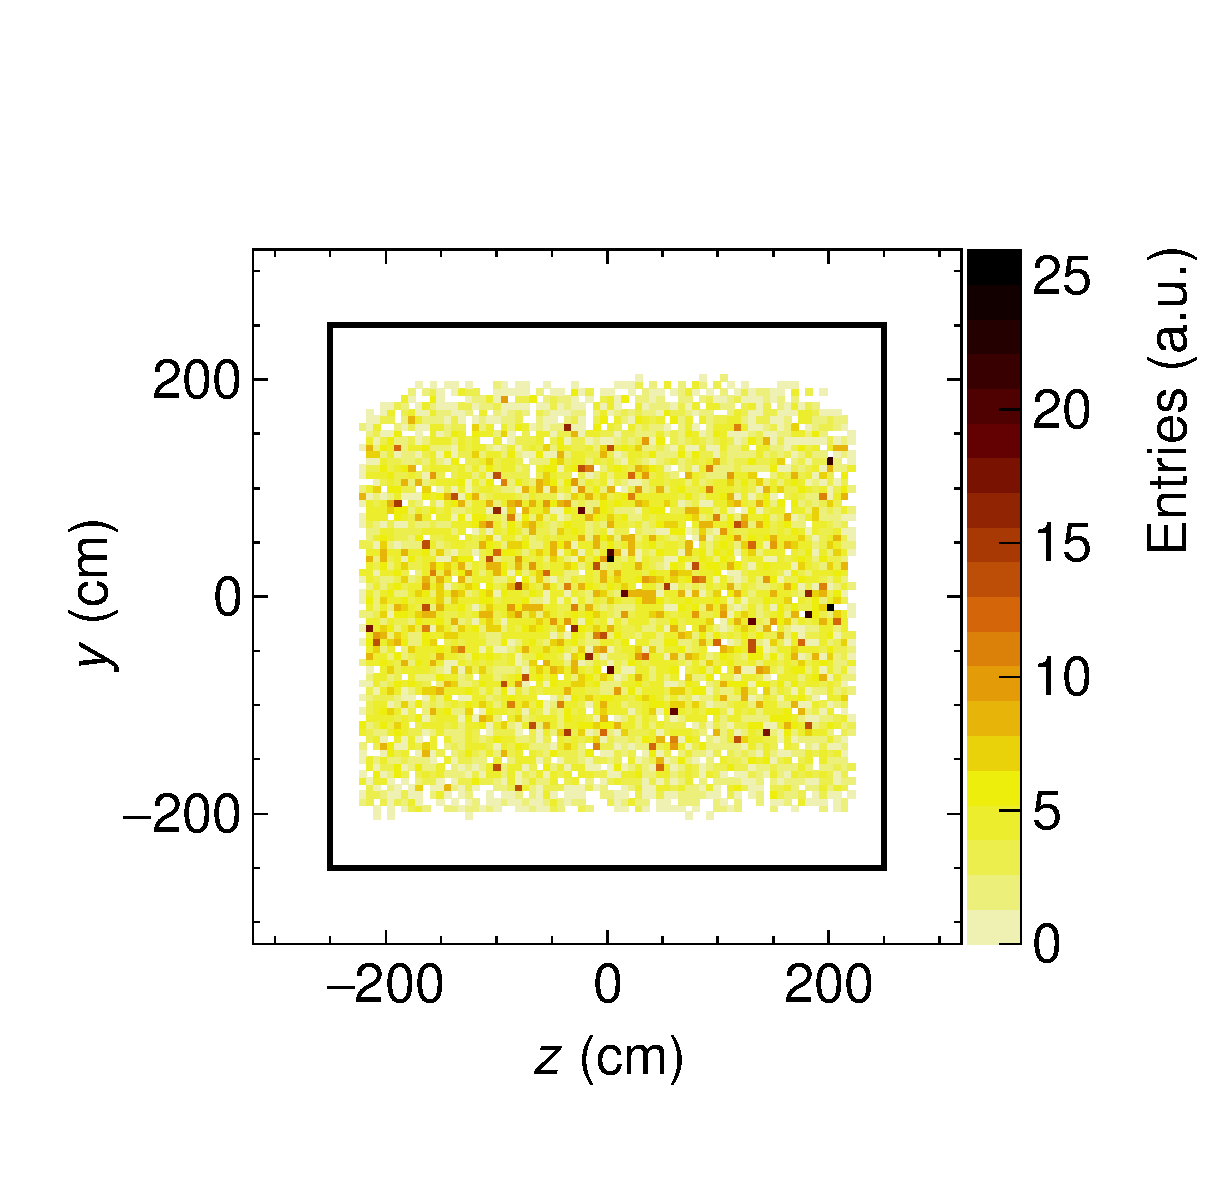
\includegraphics[width=\textwidth]{figures/ch4-KF_NDGArLite/Toy/YZ_view.eps}
         \caption{}
         \label{fig:YZViewGArLite}
     \end{subfigure}
     \begin{subfigure}[b]{0.48\textwidth}
         \centering
         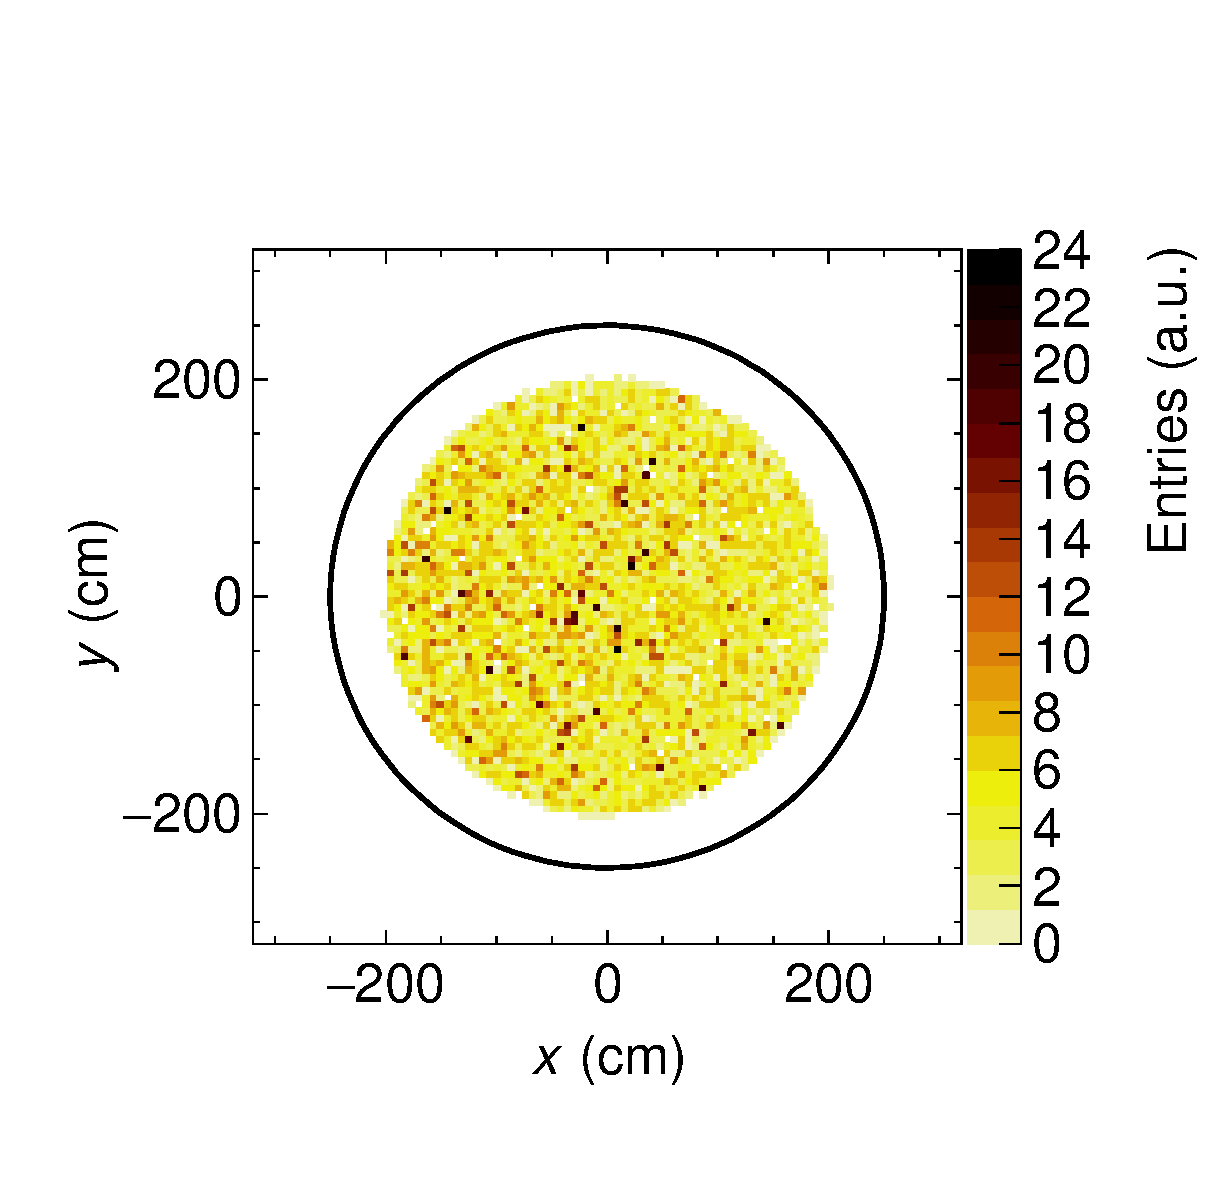
\includegraphics[width=\textwidth]{figures/ch4-KF_NDGArLite/Toy/XY_view.eps}
         \caption{}
         \label{fig:XYViewGArLite}
     \end{subfigure}
        \caption{Event display showing 8 muon tracks from the simulated sample in (a) $zy$ and (b) $xy$ view. The edges of the cylindrical tracking region are outlined in black, while the tracking planes are outlined in blue. The simulated trajectories are traced in black, while the plane hits are highlighted with red markers.} \label{fig:ViewGArLite}
\end{figure}

The difference between the two samples stems from the reconstruction. In both cases the \texttt{Seed} algorithm followed by the KF algorithm are used sequentially, but only in the second case the Energy Loss and Multiple Scattering corrections are applied to both portions of the algorithm (i.e. the \texttt{Seed} algorithm and the \texttt{KF-Lite}). The purpose of comparing the two samples is to show the impact that the energy loss and multiple scattering corrections have on the reconstruction, as well as to verify that the simulation and reconstruction algorithms are internally consistent. We denote the sample in which the material budget corrections are not applied as the Non Corrected Sample or NC Sample and the other sample as the Corrected Sample or C Sample.

An example event display showing 8 muon tracks from the simulated sample are shown in in Fig. \ref{fig:ViewGArLite} both in a $zy$ and $xy$ view. The edges of the cylindrical tracking region are outlined in black, while the tracking planes are outlined in blue. The simulated trajectories are traced in black, while the plane hits are highlighted with red markers.

\begin{figure}[t]
     \centering
     \begin{subfigure}[b]{0.48\textwidth}
         \centering
         \includegraphics[width=\textwidth]{figures/ch4-KF_NDGArLite/Toy/LengthAllTall.eps}
         \caption{}
         \label{fig:ToyGArLite_L}
     \end{subfigure}
     \begin{subfigure}[b]{0.48\textwidth}
         \centering
         \includegraphics[width=\textwidth]{figures/ch4-KF_NDGArLite/Toy/NPointsAllTall.eps}
         \caption{}
         \label{fig:ToyGArLite_N}
     \end{subfigure}
          \begin{subfigure}[b]{0.48\textwidth}
         \centering
         \includegraphics[width=\textwidth]{figures/ch4-KF_NDGArLite/Toy/pAllTall.eps}
         \caption{}
         \label{fig:ToyGArLite_p}
     \end{subfigure}
     \begin{subfigure}[b]{0.48\textwidth}
         \centering
         \includegraphics[width=\textwidth]{figures/ch4-KF_NDGArLite/Toy/NPlanesAllTall.eps}
         \caption{}
         \label{fig:ToyGArLite_planes}
     \end{subfigure}
        \caption{Properties of the particles simulated for the Toy Monte Carlo NC and C samples: (a) length of the particle tracks $L$ (cm) measured as the summed distances between the hit clusters; (b) number of hit clusters belonging to the tracks $N$; (c) initial momentum of the particles $p$ (GeV/$c$); (d) total number of tracking planes traversed by the particle $N_\text{planes}.$} \label{fig:ToyGArLite_prop}
\end{figure}

\begin{figure}[t]
     \centering
     \begin{subfigure}{0.32\textwidth}
         \centering
         \includegraphics[width=\textwidth]{figures/ch4-KF_NDGArLite/Toy/NoCorr/UnitSeed_p0.eps}
         \caption{}
         \label{fig:resp0Seed_GArLite_NoCorr}
     \end{subfigure}
     \begin{subfigure}{0.32\textwidth}
         \centering
         \includegraphics[width=\textwidth]{figures/ch4-KF_NDGArLite/Toy/NoCorr/UnitSeed_p1.eps}
         \caption{}
         \label{fig:resp1Seed_GArLite_NoCorr}
     \end{subfigure}
    \begin{subfigure}{0.32\textwidth}
         \centering
         \includegraphics[width=\textwidth]{figures/ch4-KF_NDGArLite/Toy/NoCorr/UnitSeed_p2.eps}
         \caption{}
         \label{fig:resp2Seed_GArLite_NoCorr}
     \end{subfigure}
          \begin{subfigure}{0.32\textwidth}
         \centering
         \includegraphics[width=\textwidth]{figures/ch4-KF_NDGArLite/Toy/NoCorr/UnitSeed_p3.eps}
         \caption{}
         \label{fig:resp3Seed_GArLite_NoCorr}
     \end{subfigure}
     \begin{subfigure}{0.32\textwidth}
         \centering
         \includegraphics[width=\textwidth]{figures/ch4-KF_NDGArLite/Toy/NoCorr/UnitSeed_p4.eps}
         \caption{}
         \label{fig:resp4Seed_GArLite_NoCorr}
     \end{subfigure}
        \caption{Pull distributions for the \texttt{Seed} algorithm over the Non-Corrected sample. All distributions were fitted to a Gaussian function. Results for parameters $s_0$ to $s_4$ (i.e. $y$, $x$, $\sin\phi$, $\tan\lambda$ and $q/p_{\text{T}}$) are shown from left to right and labeled from (a) to (e) accordingly. }
        \label{fig:ToyUnitSeed_GArLite_NoCorr}
\end{figure}

Some key quantities that describe the properties of the two samples are shown in Fig. \ref{fig:ToyGArLite_prop}. Fig. \ref{fig:ToyGArLite_L} shows the distribution of the tracks lengths $L$ in cm's defined as the total distance between the scintillator planes hit clusters. The distribution shows two clear peaks: one between 100 and 200 cm's and the other around 400cm. The two-peak distribution is easily explained by considering the disposition of the tracking planes in the 6-plane geometry for ND-GAr-Lite. In the 6-planes geometry the first 5 planes are disposed within the first 200 cm of the detector cylinder in the beam direction, while the last one is set 200 cm apart from all the others. This is confirmed by Fig. \ref{fig:ToyGArLite_planes} which shows the number of plains which are traversed by each particle in the samples. Most tracks in the samples cross the whole 6 planes and some cross either 4 or 5, explaining the two peaks in the $L$ distribution. Additionally Fig \ref{fig:ToyGArLite_N} shows the number of hit clusters $N$ associated with each track and Fig. \ref{fig:ToyGArLite_N} the initial true momentum $p$ of the particles.


\begin{figure}[t]
     \centering
     \begin{subfigure}{0.32\textwidth}
         \centering
         \includegraphics[width=\textwidth]{figures/ch4-KF_NDGArLite/Toy/NoCorr/UnitKFEnd_p0.eps}
         \caption{}
         \label{fig:resp0KF_GArLite_NoCorr}
     \end{subfigure}
     \begin{subfigure}{0.32\textwidth}
         \centering
         \includegraphics[width=\textwidth]{figures/ch4-KF_NDGArLite/Toy/NoCorr/UnitKFEnd_p1.eps}
         \caption{}
         \label{fig:resp1KF_GArLite_NoCorr}
     \end{subfigure}
    \begin{subfigure}{0.32\textwidth}
         \centering
         \includegraphics[width=\textwidth]{figures/ch4-KF_NDGArLite/Toy/NoCorr/UnitKFEnd_p2.eps}
         \caption{}
         \label{fig:resp2KF_GArLite_NoCorr}
     \end{subfigure}
          \begin{subfigure}{0.32\textwidth}
         \centering
         \includegraphics[width=\textwidth]{figures/ch4-KF_NDGArLite/Toy/NoCorr/UnitKFEnd_p3.eps}
         \caption{}
         \label{fig:resp3KF_GArLite_NoCorr}
     \end{subfigure}
     \begin{subfigure}{0.32\textwidth}
         \centering
         \includegraphics[width=\textwidth]{figures/ch4-KF_NDGArLite/Toy/NoCorr/UnitKFEnd_p4.eps}
         \caption{}
         \label{fig:resp4KF_GArLite_NoCorr}
     \end{subfigure}
        \caption{Pull distributions for the KF algorithm over the Non-Corrected (NC) sample. All distributions were fitted to a Gaussian function. Results for parameters $s_0$ to $s_4$ (i.e. $y$, $x$, $\sin\phi$, $\tan\lambda$ and $q/p_{\text{T}}$) are shown from left to right and labeled from (a) to (e) accordingly. }
        \label{fig:ToyUnitKF_GArLite_NoCorr}
\end{figure}

\begin{figure}[t]
     \centering
     \begin{subfigure}{0.32\textwidth}
         \centering
         \includegraphics[width=\textwidth]{figures/ch4-KF_NDGArLite/Toy/Corr/UnitSeed_p0.eps}
         \caption{}
         \label{fig:resp0Seed_GArLite_Corr}
     \end{subfigure}
     \begin{subfigure}{0.32\textwidth}
         \centering
         \includegraphics[width=\textwidth]{figures/ch4-KF_NDGArLite/Toy/Corr/UnitSeed_p1.eps}
         \caption{}
         \label{fig:resp1Seed_GArLite_Corr}
     \end{subfigure}
    \begin{subfigure}{0.32\textwidth}
         \centering
         \includegraphics[width=\textwidth]{figures/ch4-KF_NDGArLite/Toy/Corr/UnitSeed_p2.eps}
         \caption{}
         \label{fig:resp2Seed_GArLite_Corr}
     \end{subfigure}
          \begin{subfigure}{0.32\textwidth}
         \centering
         \includegraphics[width=\textwidth]{figures/ch4-KF_NDGArLite/Toy/Corr/UnitSeed_p3.eps}
         \caption{}
         \label{fig:resp3Seed_GArLite_Corr}
     \end{subfigure}
     \begin{subfigure}{0.32\textwidth}
         \centering
         \includegraphics[width=\textwidth]{figures/ch4-KF_NDGArLite/Toy/Corr/UnitSeed_p4.eps}
         \caption{}
         \label{fig:resp4Seed_GArLite_Corr}
     \end{subfigure}
        \caption{Pull distributions for the \texttt{Seed} algorithm over the Corrected (C) sample. All distributions were fitted to a Gaussian function. Results for parameters $s_0$ to $s_4$ (i.e. $y$, $x$, $\sin\phi$, $\tan\lambda$ and $q/p_{\text{T}}$) are shown from left to right and labeled from (a) to (e) accordingly. }
        \label{fig:ToyUnitSeed_GArLite_Corr}
\end{figure}

\begin{figure}[t]
     \centering
     \begin{subfigure}{0.32\textwidth}
         \centering
         \includegraphics[width=\textwidth]{figures/ch4-KF_NDGArLite/Toy/Corr/UnitKFEnd_p0.eps}
         \caption{}
         \label{fig:resp0KF_GArLite_Corr}
     \end{subfigure}
     \begin{subfigure}{0.32\textwidth}
         \centering
         \includegraphics[width=\textwidth]{figures/ch4-KF_NDGArLite/Toy/Corr/UnitKFEnd_p1.eps}
         \caption{}
         \label{fig:resp1KF_GArLite_Corr}
     \end{subfigure}
    \begin{subfigure}{0.32\textwidth}
         \centering
         \includegraphics[width=\textwidth]{figures/ch4-KF_NDGArLite/Toy/Corr/UnitKFEnd_p2.eps}
         \caption{}
         \label{fig:resp2KF_GArLite_Corr}
     \end{subfigure}
          \begin{subfigure}{0.32\textwidth}
         \centering
         \includegraphics[width=\textwidth]{figures/ch4-KF_NDGArLite/Toy/Corr/UnitKFEnd_p3.eps}
         \caption{}
         \label{fig:resp3KF_GArLite_Corr}
     \end{subfigure}
     \begin{subfigure}{0.32\textwidth}
         \centering
         \includegraphics[width=\textwidth]{figures/ch4-KF_NDGArLite/Toy/Corr/UnitKFEnd_p4.eps}
         \caption{}
         \label{fig:resp4KF_GArLite_Corr}
     \end{subfigure}
        \caption{Pull distributions for the KF algorithm over the Corrected (C) sample. All distributions were fitted to a Gaussian function. Results for parameters $s_0$ to $s_4$ (i.e. $y$, $x$, $\sin\phi$, $\tan\lambda$ and $q/p_{\text{T}}$) are shown from left to right and labeled from (a) to (e) accordingly. }
        \label{fig:ToyUnitKF_GArLite_Corr}
\end{figure}

The first test performed on both the NC and C samples was a so-called pull test. A pull, $\Pi$, is defined as the difference between the true value and the reconstructed value of one of the state vector parameters $s=(y,z,\sin{\phi},\tan{\lambda},$ $ q/p_{\text{T}})=(s_0,s_1,s_2,s_3,s_4)$, normalized by the square root of the correspondent diagonal element of the covariance matrix $C_{ii}$:
\begin{equation}
\label{eq:Pull}
    \Pi_i\equiv\frac{s_i-s_i^{\text{true}}}{\sqrt{C_{ii}}}.
\end{equation}
If the covariance matrix is well defined, the distributions of the pulls should be normal, centered in 0  with $\sigma\simeq1$.

The NC sample pulls were tested, both for the \texttt{Seed} and the Kalman Filter results were fitted to a standard Gaussian distribution. Note that the pulls for the \texttt{Seed} algorithm were tested at the start of the particle trajectory, while for the Kalman Filter they were tested at the end after the full propagation. The resulting NC Sample distributions for all the state vector parameters are shown in Figs.~\ref{fig:ToyUnitSeed_GArLite_NoCorr}  and~\ref{fig:ToyUnitKF_GArLite_NoCorr} for the \texttt{Seed} and the Kalman Filter results , respectively. A very significant underestimation of the $tan\lambda$ parameter can be seen in the \texttt{Seed}  results for which we obtain a value of $\sigma$ which is roughly double the expectation. This is not corrected after the Kalman Filter propagation, for which significant underestimations can also be seen for $\sin\phi$ and $q/p_T$ parameters. This to be expected, given that the uncertainty contributions that arise from the particles' multiple scattering and energy loss have not been accounted for.

The C sample pulls were tested in an analogous manner and the resulting distributions are shown in in Figs.~\ref{fig:ToyUnitSeed_GArLite_Corr}  and~\ref{fig:ToyUnitKF_GArLite_Corr} for the \texttt{Seed} and the Kalman Filter results, respectively. The \texttt{Seed} algorithm produces slight over-estimations on the $\sin\phi$ and $\tan\lambda$ uncertainties. These imperfections however are much less significant that in the case of the NC sample and are almost completely corrected for by the propagation of the Kalman Filter for which all Pulls have $\sigma\sim 1$ and $\mu \sim 0$. This means that the energy loss and multiple scattering corrections that we apply to the algorithm are internally consistent with the simulation and allow us to produce correct estimates of the uncertainties of the reconstructed estimates of the state vector parameters.

\begin{figure}[t]
     \centering
     \begin{subfigure}[b]{0.48\textwidth}
         \centering
         \includegraphics[width=\textwidth]{figures/ch4-KF_NDGArLite/Toy/NoCorr/pRes_doublegauss.eps}
         \caption{}
         \label{fig:ToyResP_GArLite_NoCorr_Seed}
     \end{subfigure}
     \begin{subfigure}[b]{0.48\textwidth}
         \centering
         \includegraphics[width=\textwidth]{figures/ch4-KF_NDGArLite/Toy/NoCorr/pResKF_doublegauss.eps}
         \caption{}
         \label{fig:ToyResP_GArLite_NoCorr_KF}
     \end{subfigure}
        \caption{Momentum fractional residuals $R=p_{\text{reco}}/p_{\text{true}} - 1$ for the (a) \texttt{Seed} and (b) Kalman Filter algorithms in the NC Toy Monte Carlo sample. In both cases the distributions were fitted with a double Gaussian function defining a core and a tail distributions.} \label{fig:ToyResP_GArLite_NoCorr}
\end{figure}

For both the NC and C we focused as figures of merit of the total momentum resolution and bias. Both of these quantities can be defined as the $\sigma$ and $\mu$ of a Gaussian fit applied to the momentum fractional residuals:
\begin{equation}
    \label{eq:MomentumRes}
    R = \frac{p_{\text{reco}}}{p_{\text{true}}} - 1.
\end{equation}
In Fig. \ref{fig:ToyResP_GArLite_NoCorr} we show the momentum fractional residual distributions obtained for the \texttt{Seed} and KF algorithms in the NC sample where the Energy loss and multiple scattering corrections haven't been applied. In both cases the distributions were fitted with a double Gaussian function defining core and tails sub-sets. The \texttt{Seed} algorithm is shown produce a significant negative bias $\mu_\text{core}=(-3.1\pm0.1)\%$ in the momentum estimation. This is due to an underestimation of the momentum brought by the lack of energy loss correction imparted to the algorithm's estimate. Similarly the Kalman Filter residuals shows a positive but much less significant bias $\mu_\text{core}=(0.6\pm0.1)\%$. The opposite direction of the bias is to be expected, since the estimate is produced at the end of the particle trajectory rather than at the start.

\begin{figure}[t]
     \centering
     \begin{subfigure}[b]{0.48\textwidth}
         \centering
         \includegraphics[width=\textwidth]{figures/ch4-KF_NDGArLite/Toy/Corr/pRes_doublegauss.eps}
         \caption{}
         \label{fig:ToyResP_GArLite_Corr_Seed}
     \end{subfigure}
     \begin{subfigure}[b]{0.48\textwidth}
         \centering
         \includegraphics[width=\textwidth]{figures/ch4-KF_NDGArLite/Toy/Corr/pResKF_doublegauss.eps}
         \caption{}
         \label{fig:ToyResP_GArLite_Corr_KF}
     \end{subfigure}
        \caption{Momentum fractional residuals $R=p_{\text{reco}}/p_{\text{true}} - 1$ for the (a) \texttt{Seed} and (b) Kalman Filter algorithms in the NC Toy Monte Carlo sample. Similar to Fig. \ref{fig:ToyResP_GArLite_Corr}.} \label{fig:ToyResP_GArLite_Corr}
\end{figure}

In Fig. \ref{fig:ToyResP_GArLite_Corr} we show the momentum fractional residual distributions obtained for the \texttt{Seed} and KF algorithms in the C sample where the Energy loss and multiple scattering corrections have been applied. In both cases the distributions were fitted with a double Gaussian function analogously to what was done for the NC sample. The bias seen for \texttt{Seed} algorithm in the NC sample is now almost completely corrected having $\mu_\text{core}=(0.3\pm0.1)\%$. Similarly the Kalman Filter residuals shows no bias having  $\mu_\text{core}=(0.0\pm 0.1)\%$ . The energy loss correction that we apply to both algorithm is shown to be perfectly consistent with the simulation.

\begin{figure}[t]
     \centering
     \begin{subfigure}[b]{0.42\textwidth}
         \centering
         \includegraphics[width=\textwidth]{figures/ch4-KF_NDGArLite/Toy/RespVSN.eps}
         \caption{}
         \label{fig:ToyResPVSN_GArLite_Res}
     \end{subfigure}
     \begin{subfigure}[b]{0.42\textwidth}
         \centering
         \includegraphics[width=\textwidth]{figures/ch4-KF_NDGArLite/Toy/BiaspVSN.eps}
         \caption{}
         \label{fig:ToyResPVSN_GArLite_Bias}
     \end{subfigure}
     \begin{subfigure}[b]{0.42\textwidth}
         \centering
         \includegraphics[width=\textwidth]{figures/ch4-KF_NDGArLite/Toy/RespVSp.eps}
         \caption{}
         \label{fig:ToyResPVSp_GArLite_Res}
     \end{subfigure}
     \begin{subfigure}[b]{0.42\textwidth}
         \centering
         \includegraphics[width=\textwidth]{figures/ch4-KF_NDGArLite/Toy/BiaspVSp.eps}
         \caption{}
         \label{fig:ToyResPVSp_GArLite_Bias}
     \end{subfigure}
        \caption{Relative momentum resolution $\sigma$ and bias $\mu$ as a function of (a),(b) the number of hit clusters belonging to the track and (c),(d) the initial true momentum of the particle. The results for the NC sample are shown in black while for the C sample are shown in blue } \label{fig:ToyResPVS_GArLite}
\end{figure}



For a more complete view of the results we also show the relative momentum resolution and bias produced by the Kalman Filter algorithm as a function of some key track properties. The results for the NC and C sample are shown in black and blue respectively.  In Fig. \ref{fig:ToyResPVS_GArLite} we show the two quantities as a function of the number of hit clusters belonging to the track $N$ (Figs. \ref{fig:ToyResPVSN_GArLite_Bias} and \ref{fig:ToyResPVSN_GArLite_Res})the particle's initial true momentum $p^\texttt{true}$ (Figs. \ref{fig:ToyResPVSp_GArLite_Bias} and \ref{fig:ToyResPVSp_GArLite_Res}). Note that in both of these cases the $\mu$ and $\sigma$ values are taken from a simple Gaussian fit, rather that a double Gaussian fit as was done for Figs. \ref{fig:ToyResP_GArLite_NoCorr} and \ref{fig:ToyResP_GArLite_Corr}. It is clear from a direct comparison of the two samples that while the results are comparable in terms of resolution, a significant bias correction in the momentum reconstruction is achieved by the application of the energy loss correction step to the Kalman Filter. 

The dependency of the momentum resolution on $p$ and $N$ can be explained by  adapting the Gluckstern formulas that we quoted for the expected resolution of the $1/p_{\text{T}}$ factor in Eqs.[Ref-needed] and [ref-needed]. Using error propagation the new formulas can then be written as:
\begin{equation}\label{eq:sigmaNptot}
\frac{\sigma_{\text{H}}(p)}{p}=\frac{\cos\lambda \ p  \ \sigma_{r\phi}}{0.3 BL_\textrm{Arm}^2}\sqrt{\frac{720}{N+4}}.
\end{equation}
\begin{equation}\label{eq:sigmaMSptot}
\frac{\sigma_{\text{MS}}(p)}{p}=\frac{0.016 \ (\textrm{GeV}/c)}{0.3 B l\beta \cos \lambda}\sqrt{\frac{l}{X_0}},
\end{equation}
where $\sigma_{\text{H}}(p)$ is the point resolution component of the total momentum resolution and $\sigma_{\text{MS}}(p)$ is the multiple scattering component. The total resolution is expected to be:
\begin{equation}
    \sigma_\text{tot}(p)=\sqrt{\sigma_\text{H}^2+\sigma_\text{MS}^2}
\end{equation}
The multiple scattering component $\sigma_\text{MS}$ is dominant at lower momenta, while the hit component $\sigma_\text{H}$. This can be clearly seen in Fig. \ref{fig:ToyResPVSp_GArLite_Res} where at lower momenta the resolution has an inverse proportionality on the momentum, which directly derives from the $\beta$ at the denominator present in Eq. \ref{eq:sigmaMSptot}, while at higher momenta the direct proportionality seen in Eq. \ref{eq:sigmaNptot} dominates. In Fig. \ref{fig:ToyResPVSN_GArLite_Res} on the other hand we clearly see the $\propto 1/\sqrt{N}$ dependency that we expect from Eq. \ref{eq:sigmaNptot}

\section{The GArSoft simulation studies}
\label{Sec:MC-Studies-Lite}

\begin{figure}[t]
     \centering
     \includegraphics[width=0.6\textwidth]{figures/ch4-KF_NDGArLite/MC/EvtDisplay.png}
     \caption{GArsoft event display showing a muon produced with the particle gun feature and used for the Lite-1 and Lite-2 studies. The layout of the tracker area is outlined in white and the trajectory of the muon is shown in blue. }
        \label{fig:GArLiteMuonEvent}
\end{figure} 

The GArSoft software suite described in Section \ref{Sec:GArSoft_Lite} was used to construct a particle sample to test the performance of the new Kalman Filter algorithm and compare it to the \texttt{ILRM} algorithm which represented the standard reconstruction fit at the time. The simulation was conducted using the Geant4 particle gun tool described in Section [Ref-Needed] and using the 6-plane ND-GAr-Lite geometry. The sample was mono-energetic, containing muons having the same initial momenta $p=1\ \text{GeV}/c$ and starting position in the front and center of the first scintillator tracking planes.  All particles were simulated to have a forward going momentum, with randomized small $y$ and $z$ components. These limited initial conditions were chosen for the simplicity of production as well as implementation with the new Kalman Filter algorithm. They were also chosen to be a relatively close match with the conditions of muons coming from ND-LAr which are the main sample of interest for ND-GAr-Lite. An example GArSoft event display for one of these simulated events is shown in Fig. \ref{fig:GArLiteMuonEvent} .  

Similarly to the Toy MC studies described in Section [ref-needed] many aspects of the reconstruction algorithm could be switched on and off modularly, in order to be tested individually. These feature include the energy loss and multiple scattering corrections which can be applied to both the seeding algorithm and the Kalman Filter. Additionally two separate types of seeding algorithm were implemented: the \texttt{Seed} algorithm as well as the \texttt{ILRM} algorithm. All the different testing conditions are summarized in Table in the Appendix alongside those constructed with the Toy Monte Carlo tool. 

\begin{figure}[t]
     \centering
     \begin{subfigure}[b]{0.48\textwidth}
         \centering
         \includegraphics[width=\textwidth]{figures/ch4-KF_NDGArLite/MC/LengthAllTall.eps}
         \caption{}
         \label{fig:MCGArLite_L}
     \end{subfigure}
     \begin{subfigure}[b]{0.48\textwidth}
         \centering
         \includegraphics[width=\textwidth]{figures/ch4-KF_NDGArLite/MC/NPointsAllTall.eps}
         \caption{}
         \label{fig:MCGArLite_N}
     \end{subfigure}
        \caption{Properties of the particles simulated for the GArSoft Lite-1 and Lite-2 samples: (a) length of the particle tracks $L$ (cm) measured as the summed distances between the hit clusters; (b) number of hit clusters belonging to the tracks $N$.} \label{fig:MCGArLite_prop}
\end{figure}

\begin{figure}[t]
     \centering
     \begin{subfigure}{0.32\textwidth}
         \centering
         \includegraphics[width=\textwidth]{figures/ch4-KF_NDGArLite/MC/ALICE+KF/UnitSeed_p0.eps}
         \caption{}
         \label{fig:resp0Seed_GArLite_ALICE+KF}
     \end{subfigure}
     \begin{subfigure}{0.32\textwidth}
         \centering
         \includegraphics[width=\textwidth]{figures/ch4-KF_NDGArLite/MC/ALICE+KF/UnitSeed_p1.eps}
         \caption{}
         \label{fig:resp1Seed_GArLite_ALICE+KF}
     \end{subfigure}
    \begin{subfigure}{0.32\textwidth}
         \centering
         \includegraphics[width=\textwidth]{figures/ch4-KF_NDGArLite/MC/ALICE+KF/UnitSeed_p2.eps}
         \caption{}
         \label{fig:resp2Seed_GArLite_ALICE+KF}
     \end{subfigure}
          \begin{subfigure}{0.32\textwidth}
         \centering
         \includegraphics[width=\textwidth]{figures/ch4-KF_NDGArLite/MC/ALICE+KF/UnitSeed_p3.eps}
         \caption{}
         \label{fig:resp3Seed_GArLite_ALICE+KF}
     \end{subfigure}
     \begin{subfigure}{0.32\textwidth}
         \centering
         \includegraphics[width=\textwidth]{figures/ch4-KF_NDGArLite/MC/ALICE+KF/UnitSeed_p4.eps}
         \caption{}
         \label{fig:resp4Seed_GArLite_ALICE+KF}
     \end{subfigure}
        \caption{Pull distributions for the \texttt{Seed} algorithm over the ALICE+KF sample. All distributions were fitted to a Gaussian function. Results for parameters $s_0$ to $s_4$ (i.e. $y$, $x$, $\sin\phi$, $\tan\lambda$ and $q/p_{\text{T}}$) are shown from left to right and labeled from (a) to (e) accordingly. }
        \label{fig:MCUnitSeed_GArLite_ALICE+KF}
\end{figure}

In this Section we focus on the results obtained for the two most complete and best performing combinations of the algorithm correspond to samples 15.5.2c and 15.5.6c in Table \ref{Tab:Lite} in the Appendix. In both cases we use the same Kalman Filter algorithm and the full set of material budget corrections are applied, but the two samples are differentiated by the seeding strategy: the ALICE 3-point method in the first case, the ILRM in the second. These two test sample conditions will be referred to as sample Lite-1 and sample Lite-2 respectively. Some key properties of the particle tracks in the samples are shown in Fig. \ref{fig:MCGArLite_prop}, specifically the number of hit clusters belonging to the particle track $N$ and the length of the tracks $L$ as defined in Sec. \ref{Sec:ToyMCTests-Lite}. Comparing the properties with those shown in Fig. \ref{fig:ToyGArLite_prop} it's clear that the Toy Monte Carlo simulation produced results that are very close to the more complete simulation available in GArSoft.

Similarly to what was done within the Toy Monte Carlo study pull-tests were performed for both the seeding algorithm (which include both the \texttt{Seed} and the \texttt{ILRM}) and the Kalman Filter algorithm after the full propagation. Note that in this case both results are taken at the start of the muon track, for ease of comparison with the GArSoft reconstruction results. This because, while the Kalman Filter was always applied twice, producing estimates at both end of the track, the original \texttt{ILRM} reconstruction was only applied once, producing a single estimation at the start of the track. 


\begin{figure}[t]
     \centering
     \begin{subfigure}{0.32\textwidth}
         \centering
         \includegraphics[width=\textwidth]{figures/ch4-KF_NDGArLite/MC/ALICE+KF/UnitKFEnd_p0.eps}
         \caption{}
         \label{fig:resp0KF_GArLite_ALICE+KF}
     \end{subfigure}
     \begin{subfigure}{0.32\textwidth}
         \centering
         \includegraphics[width=\textwidth]{figures/ch4-KF_NDGArLite/MC/ALICE+KF/UnitKFEnd_p1.eps}
         \caption{}
         \label{fig:resp1KF_GArLite_ALICE+KF}
     \end{subfigure}
    \begin{subfigure}{0.32\textwidth}
         \centering
         \includegraphics[width=\textwidth]{figures/ch4-KF_NDGArLite/MC/ALICE+KF/UnitKFEnd_p2.eps}
         \caption{}
         \label{fig:resp2KF_GArLite_ALICE+KF}
     \end{subfigure}
          \begin{subfigure}{0.32\textwidth}
         \centering
         \includegraphics[width=\textwidth]{figures/ch4-KF_NDGArLite/MC/ALICE+KF/UnitKFEnd_p3.eps}
         \caption{}
         \label{fig:resp3KF_GArLite_ALICE+KF}
     \end{subfigure}
     \begin{subfigure}{0.32\textwidth}
         \centering
         \includegraphics[width=\textwidth]{figures/ch4-KF_NDGArLite/MC/ALICE+KF/UnitKFEnd_p4.eps}
         \caption{}
         \label{fig:resp4KF_GArLite_ALICE+KF}
     \end{subfigure}
        \caption{Pull distributions for the \texttt{KF} algorithm over the ALICE+KF sample. All distributions were fitted to a Gaussian function. Results for parameters $s_0$ to $s_4$ (i.e. $y$, $x$, $\sin\phi$, $\tan\lambda$ and $q/p_{\text{T}}$) are shown from left to right and labeled from (a) to (e) accordingly. }
        \label{fig:MCUnitKFEnd_GArLite_ALICE+KF}
\end{figure}

\begin{figure}[t]
     \centering
     \begin{subfigure}{0.32\textwidth}
         \centering
         \includegraphics[width=\textwidth]{figures/ch4-KF_NDGArLite/MC/ILRM+KF/UnitSeed_p0.eps}
         \caption{}
         \label{fig:resp0Seed_GArLite_ILRM+KF}
     \end{subfigure}
     \begin{subfigure}{0.32\textwidth}
         \centering
         \includegraphics[width=\textwidth]{figures/ch4-KF_NDGArLite/MC/ILRM+KF/UnitSeed_p1.eps}
         \caption{}
         \label{fig:resp1Seed_GArLite_ILRM+KF}
     \end{subfigure}
    \begin{subfigure}{0.32\textwidth}
         \centering
         \includegraphics[width=\textwidth]{figures/ch4-KF_NDGArLite/MC/ILRM+KF/UnitSeed_p2.eps}
         \caption{}
         \label{fig:resp2Seed_GArLite_ILRM+KF}
     \end{subfigure}
          \begin{subfigure}{0.32\textwidth}
         \centering
         \includegraphics[width=\textwidth]{figures/ch4-KF_NDGArLite/MC/ILRM+KF/UnitSeed_p3.eps}
         \caption{}
         \label{fig:resp3Seed_GArLite_ILRM+KF}
     \end{subfigure}
     \begin{subfigure}{0.32\textwidth}
         \centering
         \includegraphics[width=\textwidth]{figures/ch4-KF_NDGArLite/MC/ILRM+KF/UnitSeed_p4.eps}
         \caption{}
         \label{fig:resp4Seed_GArLite_ILRM+KF}
     \end{subfigure}
        \caption{Pull distributions for the \texttt{Seed} algorithm over the ILRM+KF sample. All distributions were fitted to a Gaussian function. Results for parameters $s_0$ to $s_4$ (i.e. $y$, $x$, $\sin\phi$, $\tan\lambda$ and $q/p_{\text{T}}$) are shown from left to right and labeled from (a) to (e) accordingly. }
        \label{fig:MCUnitSeed_GArLite_ILRM+KF}
\end{figure}

\begin{figure}[t]
     \centering
     \begin{subfigure}{0.32\textwidth}
         \centering
         \includegraphics[width=\textwidth]{figures/ch4-KF_NDGArLite/MC/ILRM+KF/UnitKFEnd_p0.eps}
         \caption{}
         \label{fig:resp0KF_GArLite_ILRM+KF}
     \end{subfigure}
     \begin{subfigure}{0.32\textwidth}
         \centering
         \includegraphics[width=\textwidth]{figures/ch4-KF_NDGArLite/MC/ILRM+KF/UnitKFEnd_p1.eps}
         \caption{}
         \label{fig:resp1KF_GArLite_ILRM+KF}
     \end{subfigure}
    \begin{subfigure}{0.32\textwidth}
         \centering
         \includegraphics[width=\textwidth]{figures/ch4-KF_NDGArLite/MC/ILRM+KF/UnitKFEnd_p2.eps}
         \caption{}
         \label{fig:resp2KF_GArLite_ILRM+KF}
     \end{subfigure}
          \begin{subfigure}{0.32\textwidth}
         \centering
         \includegraphics[width=\textwidth]{figures/ch4-KF_NDGArLite/MC/ILRM+KF/UnitKFEnd_p3.eps}
         \caption{}
         \label{fig:resp3KF_GArLite_ILRM+KF}
     \end{subfigure}
     \begin{subfigure}{0.32\textwidth}
         \centering
         \includegraphics[width=\textwidth]{figures/ch4-KF_NDGArLite/MC/ILRM+KF/UnitKFEnd_p4.eps}
         \caption{}
         \label{fig:resp4KF_GArLite_ILRM+KF}
     \end{subfigure}
        \caption{Pull distributions for the \texttt{KF} algorithm over the ILRM+KF sample. All distributions were fitted to a Gaussian function. Results for parameters $s_0$ to $s_4$ (i.e. $y$, $x$, $\sin\phi$, $\tan\lambda$ and $q/p_{\text{T}}$) are shown from left to right and labeled from (a) to (e) accordingly. }
        \label{fig:MCUnitKFEnd_GArLite_ILRM+KF}
\end{figure}

The pull distributions for all the state vector parameters obtained using the \texttt{Seed} algorithm are shown in Fig. \ref{fig:MCUnitSeed_GArLite_ALICE+KF}. All pulls are fitted with simple Gaussian distribution showing no biases and $\sigma\sim1$. A somewhat significant over-estimation of the uncertainties can be seen for parameters $s_2=\sin\phi$ and $s_3=\tan\lambda$. This was also seen in Fig. \ref{fig:ToyUnitSeed_GArLite_Corr} and is consistent with previous test results. 

In Fig. \ref{fig:MCUnitKFEnd_GArLite_ALICE+KF} we show the pulls obtained after the full propagation of the Kalman Filter algorithm. In this case the over-estimation seen for $s_2=\sin\phi$ and $s_3=\tan\lambda$ is fully corrected for, but a slight over-estimation on parameter $s_4=q/p_\texttt{T}$ which was not seen in the equivalent Toy Monte Carlo test (see Fig. \ref{fig:ToyUnitKF_GArLite_Corr}) is introduced. 

To produce these results an ad-hoc correction to the multiple scattering correction step of the Kalman Filter reconstruction was introduced. This correction is applied in those propagation steps where the two consecutive hit clusters belong to different tracking planes and the particle is partially moving between them. In the Toy Monte Carlo the space between the tracking planes was simulated to be completely empty, while in the more realistic geometry used by GArSoft, they are filled with air at atmospheric pressure. The propagation of the particles in these passive portions of the detector produces additional multiple scattering uncertainties that, while small compared to the impact of the scintillator planes, are not completely negligible. In order to compensate for this underestimation a multiplicative factor of 4 is applied to the $Q$ matrix described in Eq. \ref{eq:Q}. This factor was found by trial and error and was shown to produce the best pulls overall. A more proper treatment would have been to apply an additional correction step calculating the length of the trajectory between the planes and using the material properties of air. However this was not attempted as the ad hoc correction already showed satisfactory results. 

The pull distributions obtained using the \texttt{ILRM} algorithm as the seeding algorithm  are shown in Fig. \ref{fig:MCUnitSeed_GArLite_ILRM+KF}. While the results don't show any bias the $\sigma$ values for parameters $s_2=\sin\phi$, $s_3=\tan\lambda$ and $s_4=q/p_\text{T}$ are largely over-estimated by a factor of $\sim2$. This is in line with the expectations for the reasons outlined in Section \ref{Sec:SeedingLite}. Specifically the fact that the method used for the calculation of the $C_0$ matrix is only valid if just three points are used for the estimate, as it was intended for the \texttt{Seed} method. 

After the full propagation of the Kalman Filter algorithm the over-estimation in the pulls are largely corrected for. This can be seen in Fig. \ref{fig:MCUnitKFEnd_GArLite_ILRM+KF} were the pulls are shown for the Kalman Filter algorithm where the \texttt{ILRM} seed is applied. All the $\sigma$ are very close to 1 with the exception of $s_4=q/p_\text{T}$ for which a somewhat significant under-estimation is seen. Note that the ad-hoc treatment needed for the propagation in air described for the Lite-1 sample was also used in this case. 

\begin{figure}[t]
     \centering
     \begin{subfigure}{0.32\textwidth}
         \centering
         \includegraphics[width=\textwidth]{figures/ch4-KF_NDGArLite/MC/ALICE+KF/pResKF_doublegauss.eps}
         \caption{}
         \label{fig:respKF_GArLite_ALICE+KF}
     \end{subfigure}
     \begin{subfigure}{0.32\textwidth}
         \centering
         \includegraphics[width=\textwidth]{figures/ch4-KF_NDGArLite/MC/ILRM+KF/pResKF_doublegauss.eps}
         \caption{}
         \label{fig:respKF_GArLite_ILRM+KF}
     \end{subfigure}
    \begin{subfigure}{0.32\textwidth}
         \centering
         \includegraphics[width=\textwidth]{figures/ch4-KF_NDGArLite/MC/ILRM+KF/pResILRM_doublegauss.eps}
         \caption{}
         \label{fig:respKF_GArLite_ILRM}
     \end{subfigure}
        \caption{Momentum fractional residuals $R=p_{\text{reco}}/p_{\text{true}} - 1$ for the (a) Kalman Filter paired with the 3-points method for seeding (b) Kalman Filter paired with the \texttt{ILRM} algorithm for seeding (c) the original GArSoft reconstruction which consists of the \texttt{ILRM} algorithm without any material budget corrections. In both cases the distributions were fitted with a double Gaussian function defining a core and a tail distributions.} 
        \label{fig:MCpResComparison}
\end{figure}

\begin{figure}[t]
     \centering
     \begin{subfigure}[b]{0.48\textwidth}
         \centering
         \includegraphics[width=\textwidth]{figures/ch4-KF_NDGArLite/MC/RespVSN.eps}
         \caption{}
         \label{fig:MCResPVSN_GArLite_Res}
     \end{subfigure}
     \begin{subfigure}[b]{0.48\textwidth}
         \centering
         \includegraphics[width=\textwidth]{figures/ch4-KF_NDGArLite/MC/BiaspVSN.eps}
         \caption{}
         \label{fig:MCResPVSN_GArLite_Bias}
     \end{subfigure}
        \caption{Relative momentum resolution $\sigma$ (a) and bias $\mu$ (b) as a function of the number of hit clusters belonging to the track $N$. The results are shown in black for the Lite-1 sample, in blue for the Lite-2 sample and in red for the original reconstruction produced with GArSoft.} \label{fig:MCResPVSN_GArLite}
\end{figure}

For both the Lite-1 and Lite-2 we studied the total momentum resolution and bias. Both of these quantities can be defined as the $\sigma$ and $\mu$ of a Gaussian fit applied to the momentum fractional residuals $R$ as defined in Eq. \ref{eq:MomentumRes}. 
We also compared the results with the original fit results available from GArSoft, which were produced with the \texttt{ILRM} algorithm without any material budget correction. In Fig. \ref{fig:MCpResComparison} we show the residuals distributions for the Lite-1, Lite-2 and ILRM standalone algorithms. In all cases the distributions are fitted with a double Gaussian defining a core and tail distribution as it was done for the Toy Monte Carlo results. The residuals produced with the original reconstruction method, which consist in an application of the \texttt{ILRM} algorithm without any material budget correction, are shown in Fig. \ref{fig:respKF_GArLite_ILRM} show a very clear bias that for the core distribution amount to $\mu_\text{core}= -4\%$. This bias is clearly introduced by the lack of corrections for the energy loss of the particle and it's comparable to what was seen for the NC sample \texttt{Seed} results in the Toy MC study. The residual distributions produced both with the Lite-1 and Lite-2 versions of the algorithm, which are shown in Fig. \ref{fig:respKF_GArLite_ALICE+KF} and \ref{fig:respKF_GArLite_ILRM+KF} show no significant bias, while maintaining essentially identical resolutions to the original GArSoft method.

The relative momentum resolution and bias are also shown as a function of the number of points in the particle tracks $N$ in Fig. \ref{fig:MCResPVSN_GArLite_Res} and \ref{fig:MCResPVSN_GArLite_Bias} respectively. The two quantities are taken as the $\mu$ and $\sigma$ of a simple Gaussian fit of the fractional momentum residual distributions. In black we show the results for the Lite-1 algorithm, in blue for the Lite-2 and in red for the original method. It is clear that no difference is present in terms of resolution, while for the bias the new algorithms largely outperform the old one. Additionally a somewhat significant preference is shown in terms of bias reduction with the Lite-1 algorithm compared to Lite-2. This is likely due to the better pulls produced by the seeding algorithm, which make the Kalman Filter more stable since the start of the propagation.




% \begin{figure}[!ht]
%      \centering
%      \begin{subfigure}{0.32\textwidth}
%          \centering
%          \includegraphics[width=\textwidth]{figures/ch4-KF_NDGArLite/MC/ALICE+KF/sinPhiResKF_doublegauss.eps}
%          \caption{}
%          \label{fig:sinPhiResKF_GArLite_ALICE+KF}
%      \end{subfigure}
%      \begin{subfigure}{0.32\textwidth}
%          \centering
%          \includegraphics[width=\textwidth]{figures/ch4-KF_NDGArLite/MC/ILRM+KF/sinPhiResKF_doublegauss.eps}
%          \caption{}
%          \label{fig:sinPhiResKF_GArLite_ILRM+KF}
%      \end{subfigure}
%     \begin{subfigure}{0.32\textwidth}
%          \centering
%          \includegraphics[width=\textwidth]{figures/ch4-KF_NDGArLite/MC/ILRM+KF/sinPhiResILRM_doublegauss.eps}
%          \caption{}
%          \label{fig:sinPhiResKF_GArLite_ILRM}
%      \end{subfigure}
%         \caption{p Residuals comparisons}
%         \label{fig:MCsinPhiResComparison}
% \end{figure}

% \begin{figure}[!ht]
%      \centering
%      \begin{subfigure}{0.32\textwidth}
%          \centering
%          \includegraphics[width=\textwidth]{figures/ch4-KF_NDGArLite/MC/ALICE+KF/tanlambdaResKF_doublegauss.eps}
%          \caption{}
%          \label{fig:tanlambdaResKF_GArLite_ALICE+KF}
%      \end{subfigure}
%      \begin{subfigure}{0.32\textwidth}
%          \centering
%          \includegraphics[width=\textwidth]{figures/ch4-KF_NDGArLite/MC/ILRM+KF/tanlambdaResKF_doublegauss.eps}
%          \caption{}
%          \label{fig:tanlambdaResKF_GArLite_ILRM+KF}
%      \end{subfigure}
%     \begin{subfigure}{0.32\textwidth}
%          \centering
%          \includegraphics[width=\textwidth]{figures/ch4-KF_NDGArLite/MC/ILRM+KF/tanlambdaResILRM_doublegauss.eps}
%          \caption{}
%          \label{fig:tanlambdaResKF_GArLite_ILRM}
%      \end{subfigure}
%         \caption{p Residuals comparisons}
%         \label{fig:MCtanlambdaResComparison}
% \end{figure}





